%versi 2 (8-10-2016)
\chapter{Landasan Teori}
\label{chap:teori}

\section{Gedung \cite{gedung}}
\label{sec:skripsi} 
Berdasarkan KBBI(Kamus Besar Bahasa Indonesia), gedung dapat diartikan sebagai bangunan tembok dan sebagainya yang berukuran besar sebagai tempat kegiatan, seperti perkantoran, pertemuan, perniagaan, pertunjukan, olahraga, dan sebagainya. Secara umum, gedung didefinisikan sebagai sebuah struktur buatan manusia yang terdiri atas dinding dan atap yang didirikan secara permanen di suatu tempat. Gedung juga memiliki beragam bentuk, ukuran, dan fungsi, serta telah mengalami penyesuaian sepanjang sejarah yang disebabkan oleh beberapa faktor, seperti bahan bangunan, kondisi cuaca, harga, kondisi tanah, dan alasan estetika.
\subsection{Klasifikasi Gedung}
\begin{itemize}
	\item Berdasarkan tingkat kompleksitas
	\begin{itemize}
		\item Gedung Sederhana
		
		Bangunan sederhana merupakan bangunan gedung dengan karakter sederhana, serta memiliki kompleksitas dan teknologi yang sederhana. Bangunan gedung sederhana meliputi gedung kantor dengan jumlah s.d. 2 lantai dengan luas maksimal mencapai 500m\textsuperscript{2}.
		
		\item Gedung Tidak Sederhana
		
		Bangunan gedung tidak sederhana merupakan bangunan gedung yang memiliki karakter, kompleksitas dan teknologi yang tidak sederhana. Bangunan gedung tidak sederhana. Bangunan gedung tidak sederhana meliputi gedung kantor bertingkat lebih dari 2 lantai yang memiliki luas di atas 500m\textsuperscript{2}.
		
		\item Gedung Khusus
		
		Bangunan gedung khusus merupakan bangunan gedung yang digunakan untuk kepentingan khusus, yang mempunyai tingkat kerahasiaan tinggi atau yang penyelenggaraannya dapat membahayakan lingkungan sekitar. Bangunan gedung ini memiliki kompleksitas tertentu, oleh karena itu dalam pembangunan atau pemanfaatannya membutuhkan pengelolaan dan persyaratan khusus. Bangunan gedung khusus meliputi gedung istana negara, gedung laboratorium, bangunan gedung reaktor nuklir, instalasi pertahanan dan keamanan, dan bangunan gedung sejenisnya yang ditetapkan oleh menteri.
	\end{itemize}
	
	\item Berdasarkan Fungsinya
	\begin{itemize}
		\item Gedung Rumah Tinggal 
		
		Pembuatan gedung rumah tinggal bertujuan untuk memenuhi kebutuhan manusia akan tempat tinggal. Pembuatan rumah tinggal ini harus memperhatikan faktor keamanan dan kenyamanannya. Beberapa contoh gedung rumah tinggal adalah rumah, rumah susun, asrama, mess, kontrakan dan apartemen.
		
		\item Gedung Komersial
		
		Gedung komersial didirikan untuk mendukung aktivitas komersial meliputi jual, beli, dan sewa. Gedung komersial ditujukan untuk keperluan bisnis sehingga faktor lokasi yang strategis memegang peranan penting bagi kesuksesan bangunan tersebut. Beberapa contoh gedung komersial di antaranya pasar, \textit{supermarket}, \textit{mall}, \textit{retail}, pertokoan, perkantoran dan komplek kios.
		
		\item Gedung Fasilitas Penginapan
		
		Gedung penginapan tercipta dari kebiasaan manusia yang sering melakukan aktivitas dengan berpindah-pindah tempat secara mobilitas. Keberadaan gedung ini memungkinkan seseorang bisa menyewa gedung untuk sementara waktu dengan keperluan menginap. Beberapa contoh gedung penginapan yaitu \textit{motel}, \textit{hotel}, \textit{cottage} dan wisma tamu.
	
		\item Gedung Fasilitas Pendidikan
		
		Gedung pendidikan didirikan untuk mendukung proses belajar dan mendapatkan ilmu dan pengetahuan yang baru. Beberapa contoh gedung fasilitas pendidikan adalah sekolah, universitas, perpustakaan dan gedung.
		
		\item Gedung Fasilitas Kesehatan
		
		Gedung kesehatan didirikan untuk membantu masyarakat untuk melakukan berobat agar dapat sembuh dari sakit dan dapat menjalankan aktivitasnya. Beberapa contoh dari gedung fasilitas kesehatan adalah rumah sakit, puskesmas, apotek dan pusat rehabilitasi.
		
		\item Gedung Fasilitas Peribadatan
		
		Gedung ibadah didirikan untuk memenuhi kebutuhan rohani manusia sebagai mahluk hidup yang memiliki Tuhan. Gedung peribadatan biasanya digunakan sebagai tempat beribadah dan upacara keagamaan. Beberapa contoh gedung fasilitas peribadatan adalah vihara, gereja, kelenteng, masjid dan pura.
		
		\item Gedung Fasilitas Transportasi
		
		Gedung transportasi didirikan untuk sebagai pusat dari alat transportasi tertentu. Misalnya terminal untuk tempat berhentinya bis, pelabuhan sebagai tempat menepinya kapal, stasiun untuk pemberhentian kereta api, dan bandara sebagai tempat mendaratnya pesawat. Di gedung fasilitas transportasi ini juga umumnya dilengkapi dengan fasilitas-fasilitas layanan yang menunjang alat transportasi tersebut.
		
		\item Gedung Fasilitas Budaya dan Hiburan
		
		Gedung budaya merupakan gedung yang dipakai untuk melestarikan dan atau mempertunjukkan suatu kebudayaan. Sedangkan gedung hiburan adalah gedung yang dipakai sebagai tempat menciptakan hal-hal yang menghibur. Pada gedung, hubungan antara faktor budaya dan faktor hiburan ini saling merekat dan mendukung satu sama lain. Sebagai contoh gedung pertunjukan yang menampilkan drama sarat budaya yang dapat menghibur penonton. Begitu juga dengan bioskop dan museum.
		
		\item Gedung Fasilitas Pemerintah dan Layanan Publik
		
		Gedung pemerintahan adalah gedung yang digunakan oleh pemerintah untuk menunaikan tugas dan kewajibannya. Di samping itu, gedung pemerintah ini juga dipakai sebagai gedung layanan publik misalnya dalam pengurusan data kependudukan, berkas-berkas resmi, surat perijinan, laporan pengaduan, dan lain-lain. Itu sebabnya, pembuatan gedung ini harus dirancang sedemikian rupa agar dapat mendukung kegiatan-kegiatan tersebut. Adapun contoh-contoh bangunan pemerintahan dan layanan publik yaitu kantor polisi, kantor perizinan, kantor dinas, dan balai pemerintahan.
	\end{itemize}
\end{itemize}

\subsection{Pemantauan Kesehatan Struktural \cite{struktural}}

Pemantauan kesehatan struktural atau biasa disebut Structural Health Monitoring (SHM) merupakan sebuah proses penerapan deteksi kerusakan dan karakterisasi untuk struktur teknik seperti jembatan dan bangunan. Kerusakan dalam hal ini diartikan sebagai perubahan pada material atau sifat-sifat geometris dari suatu sistem struktural yang secara negatif mempengaruhi kinerja sistem. Sifat geometris yang dimaksud adalah bangunan yang dibangun terdapat dilahan yang memiliki kemiringan sehingga sebuah gedung akan lebih mudah mengalami kerusakan. Proses pemantauan kesehatan struktural melibatkan pengamatan suatu sistem dari waktu ke waktu menggunakan pengukuran respons sampel secara berkala dari berbagai sensor (sering yang digunakan adalah \textit{accelerometer}), ekstrasi fitur yang peka terhadap kerusakan dari pengukuran ini, dan melakukan analisis statistik fitur untuk menentukan keadaan saat ini kesehatan sistem.

Salah satu contoh struktural adalah gedung. Gedung harus diukur kesehatannya untuk melihat apakah suatu gedung layak digunakan atau tidak. Gedung yang kesehatannya baik menjadi syarat untuk mendapatkan dokumen IMB (Izin Mendirikan Bangunan). Dokumen IMB merupakan dokumen dimana sebuah gedung yang akan didirikan mendapatkan izin dari pemerintah. Sebuah gedung dapat diukur kesehatannya dengan melakukan pemantauan atau \textit{monitoring} gedung. Pemantauan kesehatan gedung adalah sebuah proses pemantauan informasi kondisi dan keamanan dari sebuah gedung. Tujuan dari pemantauan kesehatan gedung ini adalah:
\begin{itemize}
	\item Memantau secara terus-menerus kondisi kesehatan gedung
	\item Mengetahui sesegera mungkin gejala-gejala tidak normal yang mungkin dapat terjadi pada sebuah gedung
	\item Mencatat perilaku-perilaku beban yang dikirim oleh gedung
	\item Sebagai sumber data untuk menganalisis dalam pengambilan keputusan dalam tindakan mencegah atau perawatan pada sebuah gedung
\end{itemize}

\subsubsection{Faktor-Faktor Kesehatan Gedung}
Kesehatan sebuah gedung dapat dilihat dari beberapa faktor. Faktor-faktor yang mempengaruhi kesehatan gedung antara lain:
\begin{itemize}
	\item Faktor Suhu
	
	Suhu merupakan salah satu faktor alam yang berpengaruh kepada kesehatan sebuah gedung. Suhu yang ekstrim dan terjadi secara terus-menerus menyebabkan kesehatan gedung menjadi rusak terutama dibagian luar gedung tersebut. Beberapa contoh komponen yang harus dilindungi karena pengaruh suhu adalah lapisan water proofing diatas atap plat beton, cat pada listplank kayu, serta cat eksterior yang sering terkena panas ataupun dingin secara terus menerus
	
	\item Faktor Air Hujan
	
	Faktor air hujan menjadi salah satu faktor yang berpengaruh kepada kesehatan suatu gedung. Air hujan dapat membuat kerusakan pada gedung dan kasus yang sering terjadi akibatnya adalah kebocoran pada gedung.
	
	\item Faktor Angin
	
	Faktor angin merupakan salah satu alam yang berpengaruh terhadap kesehatan gedung. Faktor angin dapat membuat gedung mengalami kerusakan dan salah satu komponen gedung yang sering terkena akibat angin adalah penutup atap genteng. Pada serangan angin yang kencang, menimbulkan gerakan-gerakan pada atap yang menyebabkan atap mudah bergeser satu sama lain sehingga mudah lepas jika terjadi angin kencang.
	
	\item Faktor Getaran
	
	Salah satu faktor yang dapat digunakan untuk pemantauan kesehatan gedung adalah getaran. Getaran merupakan salah satu faktor penting dalam kesehatan gedung. Getaran dalam sebuah gedung dapat berasal dari alat-alat mesin yang sedang berjalan, adanya sebuah kerusakan dalam gedung tersebut ataupun adanya sebuah pergeseran lempengan bumi atau biasa disebut gempa bumi. Getaran-getaran yang dihasilkan gedung seringkali tidak dapat dirasakan oleh manusia sehingga dibutuhkan sensor untuk mendeteksi getaran tersebut. Gedung akan dinyatakan baik dan dapat digunakan apabila getaran yang dihasilkan oleh sebuah gedung semakin kecil.
	
	\item Faktor Petir
	
	Faktor petir merupakan faktor kesehatan gedung yang jarang, tetapi kerusakan yang terjadi pada gedung akibat petir tidak dapat dianggap sepele karena kerusakan yang dihasilkan oleh petir dapat berakibat fatal diantaranya listrik pada gedung mati, jaringan telepon ataupun internet di gedung juga dapat mati.
	
	\item Faktor Hama
	
	Faktor hama merupakan faktor yang dapat mempengaruhi kesehatan gedung. Bedanya untuk faktor hama, gedung yang dapat mengalami kerusakan akibat faktor hama ini adalah gedung yang terbuat dari kayu. Salah satu contoh penyebab kerusakan akibat gedung dari faktor hama adalah rayap.
	
\end{itemize}  

\subsubsection{Sifat Kerusakan Pada Gedung}
Sifat kerusakan yang terjadi pada gedung dapat ditinjau dari pengaruh komponen tersebut hingga akibat dari kerusakan komponen sifat tersebut. Sifat-sifat kerusakan gedung dibagi menjadi tiga bagian yaitu:

\begin{itemize}
	\item \textit{Emergency}
	
	Kerusakan yang memiliki pengaruh sangat tinggi terhadap aktivitas penghuni pada gedung dan mempengaruhi komponen lain dalam,gedung tersebut. Contoh kerusakannya adalah kerusakan kran air, atap bocor, instalasi listrik.
	
	\item Urgent
	
	Kerusakan yang memiliki pengaruh tinggi terhadap aktivitas penghuni dan kerusakan komponen lainnya pada gedung. Contoh kerusakannya adalah kerusakan pada keramik yang sering dilalui, jalan berlubang.
	
	\item Normal
	
	Kerusakan kecil yang menyebabkan fungsi kurang sempurna atau penurunan tampak pada komponen yang mempunyai pengaruh kecil pada aktivitas penghuni. Contoh kerusakannya adalah cat dinding yang udah rusak.
\end{itemize}

\section{Getaran \cite{getaran}}
\label{sec:latex}
Getaran adalah suatu peristiwa gerak bolak balik secara teratur suatu benda melalui suatu titik seimbang terhadap suatu titik acuan. Keseimbangan yang dimaksud adalah suatu keadaan dimana suatu benda berada pada posisi diam jika tidak ada gaya yang bekerja pada benda tersebut.Besar kecilnya suatu getaran yang dihasilkan oleh suatu benda dipengaruhi oleh jumlah energi yang diberikan. Semakin besar energi yang diberikan maka semakin kuat getaran yang terjadi. Satu getaran sama dengan satu kali gerakan bolak balik penuh dari benda tersebut.\footnote{https://www.gurupendidikan.co.id/getaran/}

\subsubsection{Jenis getaran}
Secara umum getaran dapat diklasifikasikan menjadi beberapa jenis yaitu:
\begin{itemize}
	\item Getaran Bebas dan Paksa
	
	Jika sebuah sistem diberi inisial gangguan, sehingga akan terjadi getaran dengan sendirinya, maka getaran tersebut dinamakan \textbf{getaran bebas}. Tidak ada gaya eksternal bekerja pada sistem. Contoh dari getaran bebas adalah gerakan bolak-balik yang ada pada sebuah pendulum. Sedangkan jika sebuah sistem diberikan suatu gaya dari luar yang secara berkala (berulang-ulang) maka getaran yang dihasilkan pada sistem disebut dengan \textbf{getaran paksa}. Salah satu contoh getaran paksa adalah getaran yang dihasilkan oleh mesin yang sedang bekerja. Apabila frekuensi suatu gaya eksternal sama dengan frekuensi gaya sistem, maka akan menimbulkan resonansi. Resonansi ini dapat membahayakan suatu sistem dan menyebabkan kerusakan struktur dari bangunan.
	
	\item Getaran Teredam dan Tidak Teredam
	
	\textbf{Getaran tidak teredam} adalah getaran dimana jika tidak adanya energi dalam sebuah getaran yang hilang atau terdisipasi akibat adanya getaran atau hambatan lainnya. Sedangkan yang dimaksud dengan \textbf{getaran teredam} adalah sebuah getaran dimana mengalami pengurangan energi secara bertahap.
	
	\item Getaran Mekanis dan Nonmekanis
	
	\textbf{Getaran mekanis} adalah getaran suatu benda yang getarannya mengalami suatu pergeseran linear atau pergeseran sudut. Contoh getaran mekanis adalah getaran senar gitar pada saat dipetik, getaran pada bandul dan getaran atom pada zat padat. Sedangkan g\textbf{etaran nonmekanis} adalah suatu gerakan yang juga melibatkan adanya perubahan pada besaran-besaran fisika. Contoh dari getaran nonmekanis adalah medan listrik serta medan magnet.
	
	\item Getran Deterministik dan Acak
	
	\textbf{Getaran deterministik} adalah sebuah getaran dimana besarnya eksitasi (gaya atau gerakan) yang bekerja pada suatu sistem getaran diketahui pada waktu tertentu. \textbf{Getaran acak} adalah getaran dimana getaran atau gaya yang bekerja pada suatu sistem dihasilkan secara acak pada waktu tertentu. Contoh dari getaran acak adalah kecepatan angin, gerakan tanah selama gempa bumi.
\end{itemize}

\section{\textit{Wireless Sensor Network} \cite{wsn}} 
\label{}
\textit{Wireless Sensor Network} (WSN) merupakan jaringan nirkabel yang terdiri dari sekumpulan node sensor yang saling terhubung yang diletakan pada suatu tempat dan memiliki kemampuan untuk mengukur kondisi lingkungan sekitar (\textit{sensing}), melakukan komputasi dan dilengkapi  dengan alat komunikasi \textit{wireless} untuk komunikasi antara node sensor. \textit{Wireless Sensor Network} juga berguna untuk memantau hasil \textit{sensing} kondisi suatu lingkungan yang dilakukan oleh sensor. Selain itu WSN juga dapat mengatur data yang akan dikirimkan dan dikumpulkan di \textit{base station} atau juga dapat diteruskan ke node sensor tetangganya hingga sampai ke \textit{base station} sebagai pusat menggunakan \textit{radio transceiver} untuk dilakukan pengelolaan data(Firdaus, 2014). Bentuk radio transceiver untuk setiap node menggunakan antena internal ataupun anterna eksternal.

\subsection{Penerapan Wireless Sensor Network di berbagai bidang}
\textit{Wireless Sensor Network} pada awalnya hanya digunakan untuk melakukan ilmu komputasi saja. Semakin lama dan majunya teknologi, \textit{Wireless Sensor Network} telah digunakan untuk melakukan pemantauan ataupun pengukuran seperti di bidang militer, \textit{Wireless Sensor Network} digunakan untuk mendeteksi musuh yang ada dilautan ataupun darat. Kemudian pemanfaatannya dikembangkan untuk membantu berbagai bidang kegiatan manusia dalam kehidupan. Penerapan \textit{Wireless Sensor Network} untuk kehidupan manusia dapat dilihat pada contoh ilustrasi (Gambar~\ref{fig:penerapan})\footnote{http://eprints.polsri.ac.id/4497/3/File/20III.pdf}.Berikut adalah beberapa penerapan \textit{Wireless Sensor Network}:

\begin{itemize}
	\item Bidang Pemantauan Lingkungan
	
	
	\textit{Wireless Sensor Network} dibidang pemantauan lingkungan memiliki banyak pengaplikasian seperti untuk memantau polusi udara, mendeteksi kebakaran hutan, mendeteksi adanya bencana alam khususnya gempa, dan lain-lain.
	
	\item Bidang Kesehatan
	
	\textit{Wireless Sensor Network} dapat digunakan pada aplikasi kesehatan seperti mendeteksi kondisi manusia yang memiliki kekurangan seperti disabilitas, monitoring penggunaan obat, serta bisa juga untuk mendiagnosis sebuah penyakit.
	
	\item Bidang Transportasi
	
	Pada bidang transportasi, \textit{Wireless Sensor Network} digunakan untuk mendeteksi arus lalu lintas secara aktual yang akan dikirimkan kepada pengendara. Selain itu, juga bisa digunakan untuk mendeteksi kecepatan kendaraan yang melaju apakah melewati batas kecepatan atau tidak.
	
	\item Bidang Militer
	
	Pemanfaatan \textit{Wireless Sensor Network} di bidang militer adalah Wide Area Tracking System (WATS). WATS merupakan prototipe jaringan yang mengunakan teknologi \textit{Wireless Sensor Network} untuk mendeteksi ancaman nuklir. Pemanfaatan lainnya untuk bidang militer dapat juga digunakan untuk mendeteksi serangan dari musuh.
	
	\item Bidang Pertanian
	
	Pada bidang pertanian, Wireless Sensor Network dapat digunakan untuk membantu pengelola pertanian untuk penggunaan air, kelembaban tanah yang digunakan, pH tanah yang digunakan untuk pertanian, serta mengelola pembuangan pertanian mereka.
	
	\item Bidang Infrastruktur
	
	\textit{Wireless sensor network} juga digunakan dalam pembangunan infrastruktur. Pemanfaatan \textit{Wireless Sensor Network} biasa digunakan untuk melakukan pengamatan kondisi pembangunan infrastruktur, baik dari segi bangunan maupun geografis seperti mengukur getaran sebuah pembangunan. Penerapan WSN untuk membantu pembangunan infrastruktur dilakukan secara \textit{daily} dan \textit{real-time} untuk menjaga kondisi lingkungan selama proses pemabangunan selesai dilakukan.
\end{itemize}

\begin{figure}[H] 
	\centering  
	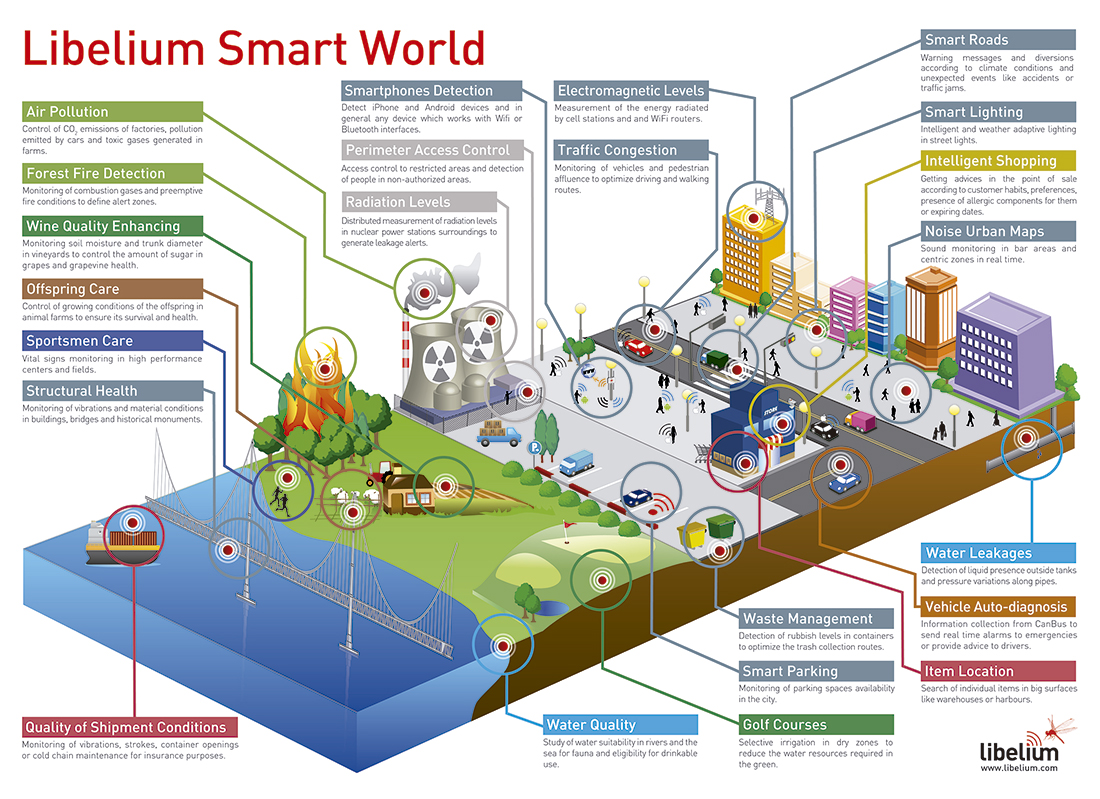
\includegraphics[scale=0.3]{penerapan}  
	\caption[Ilustrasi penerapan \textit{Wireless Sensor Network}]{Ilustrasi penerapan \textit{Wireless Sensor Network}}
	\label{fig:penerapan} 
\end{figure} 

\subsection{Struktur Node Sensor}
\label{struktur}
Node adalah salah satu titik sambungan, titik redistribusi, atau titik akhir komunikasi\footnote{http://gilang777.blogspot.com/2015/06/pengertian-node-jaringan.html}. Komponen utama node sensior antara lain \textit{controller}, \textit{transceiver}, \textit{memory}, \textit{power source}, dan sensor.(Gambar~\ref{fig:struktur}).  

\begin{figure}[H] 
	\centering  
	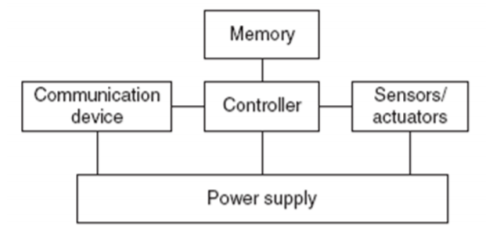
\includegraphics[scale=0.7]{struktur}  
	\caption[Struktur Node Sensor]{Struktur Node Sensor}
	\label{fig:struktur} 
\end{figure} 

\begin{itemize}
	\item Controller
	
	\textit{Controller} adalah inti utama yang ada pada node sensor. \textit{Controller} juga bertindak sebagai pengatur fungsi dari komponen-komponen lain. \textit{Controller} juga mengumpulkan data dari sensor lain dan memproses data. Pada \textit{controller} terdapat \textit{microcontroller} yang mengatur dan melakukan komputasi data. \textit{Microcontroller} lebih sering menjadi alternatif karena mengurangi penggunaan energi dan adanya sleep states yang berati hanya bagian dari \textit{controller} saja yang aktif.
	
	\item Communication Device
	
	Communication Device digunakan untuk menerima atau mengirim data antar node sensor. Communication Device membuat node sensor dapat terhubung dalam jaringan dan berkomunikasi dengan node sensor lainnya. 
	
	\item Sensor / Actuator
	
	Sensor merupakan bagian yang digunakan untuk melakukan \textit{sensing} atau pengukuran terhadap suatu keadaan lingkungan yang diamati. \textit{Actuator} berfungsi sebagai pengubah sinyal dari lingkungan menjadi besaran-besaran fisik.
	
	\item Memory
	
	\textit{Random Access Memory} (RAM) digunakan untuk menyimpan hasil sementara yang didapat dari \textit{sensing} dari sensor. RAM ini memiliki sifat \textit{volatile} yang berati jika node sensor mati atau energi habis maka data-data yang ada pada RAM akan hilang. 
	
	\item Power Supply
	
	Power Suppy digunakan sebagai sumber energi yang dibutuhkan untuk mengoperasikan fungsionalitas dari keseluruhan komponen node sensor lainnya. Penyediaan energi ini dapat memiliki dua jenis metode, yaitu \textit{storing energy} dan \textit{energy scavenging}. Metode \textit{storing energy}, sensor node menggunakan baterai sebagai energi utamanya. Jenis baterai yang digunakan dapat yang diisi ulang maupun yang tidak dapat diisi ulang. Sedangkan metode \textit{energy scavenging} digunakan saat membuat \textit{Wireless Sensor Network} yang akan digunakan dalam waktu yang lama. Pada metode \textit{energy scavenging}, node sensor menggunakan perubahan energi sebagai sumber energi utamanya. Energi yang didapat dengan metode \textit{energy scavenging} didapatkan setelah mengonversi pemanfaatan energi alam seperti cahaya matahari, air atau angin untuk dijadikan energi listrik untuk menjalankan node sensor.
	
\end{itemize}

\subsection{Arsitektur \textit{Wireless Sensor Network}}
\label{arsitektur}
Pada \textit{Wireless Sensor Network}, arsitektur yang biasanya dipakai adalah \textbf{arsitektur flat atau \textit{peer-to-peer}} dan \textit{arsitektur hierarki}. Perbedaan antara kedua jenis arsitektur adalah cara node sensor dalam berkomunikasi. Pada arsitektur \textit{flat}, node yang disebar dapat langsung mengirimkan data hasil sensing ke \textit{base station}. Sedangkan pada arsitektur \textit{hirarkikal}, node yang disebar harus mengirimkan data ke \textit{cluster head} terlebih dahulu, sebelum diteruskan ke \textit{base station}.

\begin{figure}[H] 
	\centering  
	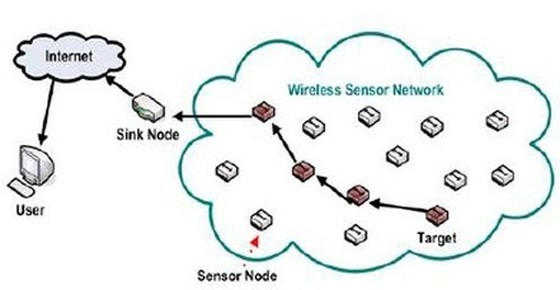
\includegraphics[scale=0.5]{arsitektur}  
	\caption[Ilustrasi penerapan \textit{Wireless Sensor Network}]{Ilustrasi penerapan \textit{Wireless Sensor Network}}
	\label{fig:arsitektur} 
\end{figure}

\begin{enumerate}[label=(\roman*)]
	\item \textbf{Arsitektur \textit{Flat} / \textit{Peer-to-Peer}}
	
	Pada arsitektur \textit{flat}, setiap node sensor yang disebar memiliki tugas dan peran yang sama dalam melakukan \textit{sensing} dan mengirimkan hasilnya ke \textit{base station}. Data hasil \textit{sensing} ini langsung dikirimkan ke \textit{base station} tanpa butuh sebuah perantara.
	
	\begin{figure}[H] 
		\centering  
		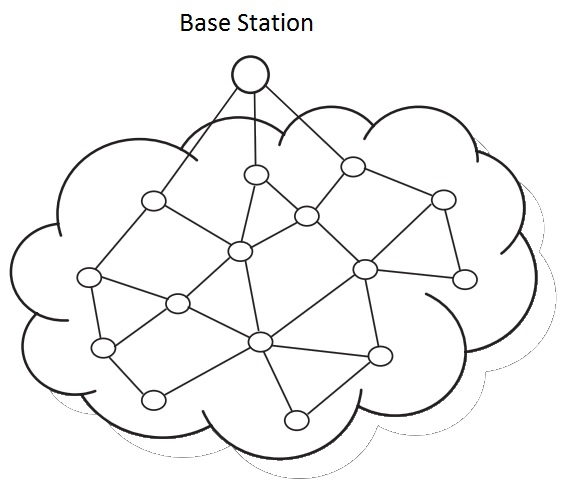
\includegraphics[scale=0.5]{flat}  
		\caption[Arsitektur \textit{flat} pada \textit{Wireless Sensor Network}]				{Arsitektur \textit{flat} pada \textit{Wireless Sensor Network}}
		\label{fig:flat} 
	\end{figure}
	
	\item \textbf{Arsitektur Hierarki}
	
	Pada arsitektur hierarki, setiap hasil \textit{sensing} dari sensor tidak langsung dikirimkan ke \textit{base station}. Melainkan setiap node sensor akan membentuk sebuah grup yang disebut dengan \textit{cluster}.Tiap \textit{cluster} terdiri dari sebuah \textit{cluster head} dan \textit{cluster member}. \textit{Cluster head} bertindak sebagai penerima data hasil sensing dari \textit{cluster member}, untuk diteruskan ke \textit{base station}. Jenis arsitektur hierarki juga dapat dibedakan berdasarkan jarak antara \textit{cluster head} dengan \textit{cluster member}. Perbedaan dari jenis ini adalah jumlah \textit{hop} yang dibutuhkan untuk mencapai tujuan yaitu \textit{base station}.
	
	\begin{itemize}
		\item \textit{Single hop}
		
		Pada arsitektur hierarki \textit{single hop}, cluster member hanya membutuhkan satu lompatan untuk mencapai ke \textit{cluster head}. Dapat dikatakan, data hasil \textit{sensing} yang diterima oleh \textit{cluster member} dapat langsung diterima oleh \textit{cluster head} tanpa adanya perantara dan dapat diteruskan ke \textit{base station}. 
		
		\begin{figure}[H] 
		\centering  
		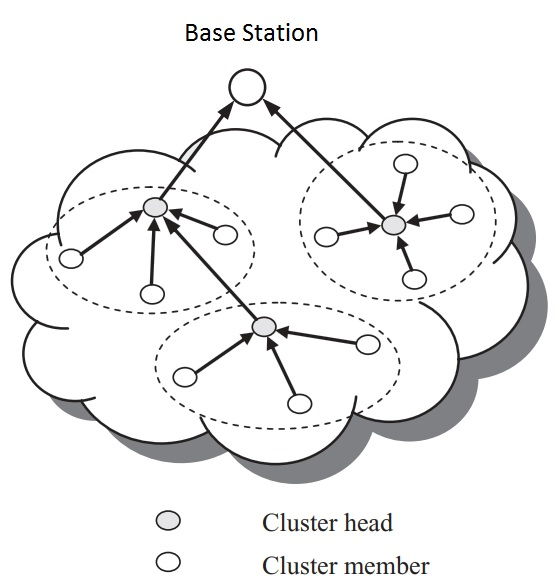
\includegraphics[scale=0.5]{hierarki}  
		\caption[Arsitektur \textit{single hop} pada \textit{Wireless Sensor Network}]{Arsitektur \textit{single hop} pada \textit{Wireless Sensor Network}}
		\label{fig:hierarki} 
	\end{figure}
		
		\item \textit{Multi hop}
		
		Pada arsitektur hierarki \textit{multi hop}, \textit{cluster member} membutuhkan lebih dari satu lompatan untuk mencapai \textit{base station}. \textit{Cluster member} akan mengirimkan data ke \textit{cluster member} yang jaraknya lebih dekat dengan \textit{cluster head} dan ini akan terus dilakukan sampai data yang dikirimkan sampai di \textit{cluster head} kemudian akan diterukan ke \textit{base station}.
		
		\begin{figure}[H] 
		\centering  
		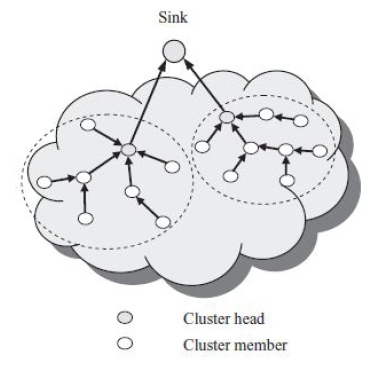
\includegraphics[scale=0.8]{multi}  
		\caption[Arsitektur \textit{multi hop} pada \textit{Wireless Sensor Network}]{Arsitektur \textit{multi hop} pada \textit{Wireless Sensor Network}}
		\label{fig:multi} 
	\end{figure}
	\end{itemize}
\end{enumerate}

\subsection{Topologi \textit{Wireless Sensor Network}}
\label{topologi}
Topologi pada \textit{wireless sensor network} memiliki beberapa jenis. Tiap jenis topologi dibedakan berdasarkan tujuan, skala jaringan dan kondisi lingkungan. Beberapa jenis topologi pada \textit{wireless sensor network} adalah topologi \textit{point-to-point} \textit{bus}, \textit{tree}, \textit{star}, \textit{ring} dan \textit{mesh}.

\begin{itemize}
	\item Topologi \textit{Point-to-Point}
	
	Topologi \textit{point-to-point} adalah topologi yang menghubungkan dua titik (Gambar~\ref{fig:poin}). Pada topologi ini dibagi menjadi dua yaitu \textit{permanent point-to-point} dan \textit{switched point-to-point}. \textit{Permanent point-to-point} adalah koneksi antara dua titik dan bersifat tidak dapat diubah (permanen). Sedangkan \textit{switched point-to-point} adalah koneksi point-to-point yang dapat dipindahkan antara node yang berbeda \footnote{http://link.springer.com/chapter/10.1007/978-1-4302-6014-14.html}.
	
	\begin{figure}[H] 
		\centering  
		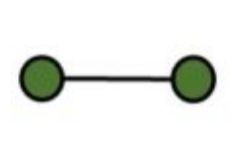
\includegraphics[scale=1]{poin}  
		\caption[Topologi \textit{point-to-point}]{Topologi \textit{point-to-point}}
		\label{fig:poin} 
	\end{figure}

	\item Topologi \textit{Bus}
	
	Topologi bus akan terdiri dari node-node yang terhubung pada sebuah jalur. Jalur ini digunakan oleh node-node untuk saling berkomunikasi (Gambar~\ref{fig:bus}). Sifat komunikasi pada jalur ini adalah satu arah, dimana komunikasi node dilakukan secara bergantian. Topologi ini sederhana dan mudah untuk diimplementasikan. Kekurangan dari topologi ini adalah apabila jalur mengalami kerusakan maka setiap node tidak dapat melakukan komunikasi lagi.
	
	\begin{figure}[H] 
		\centering  
		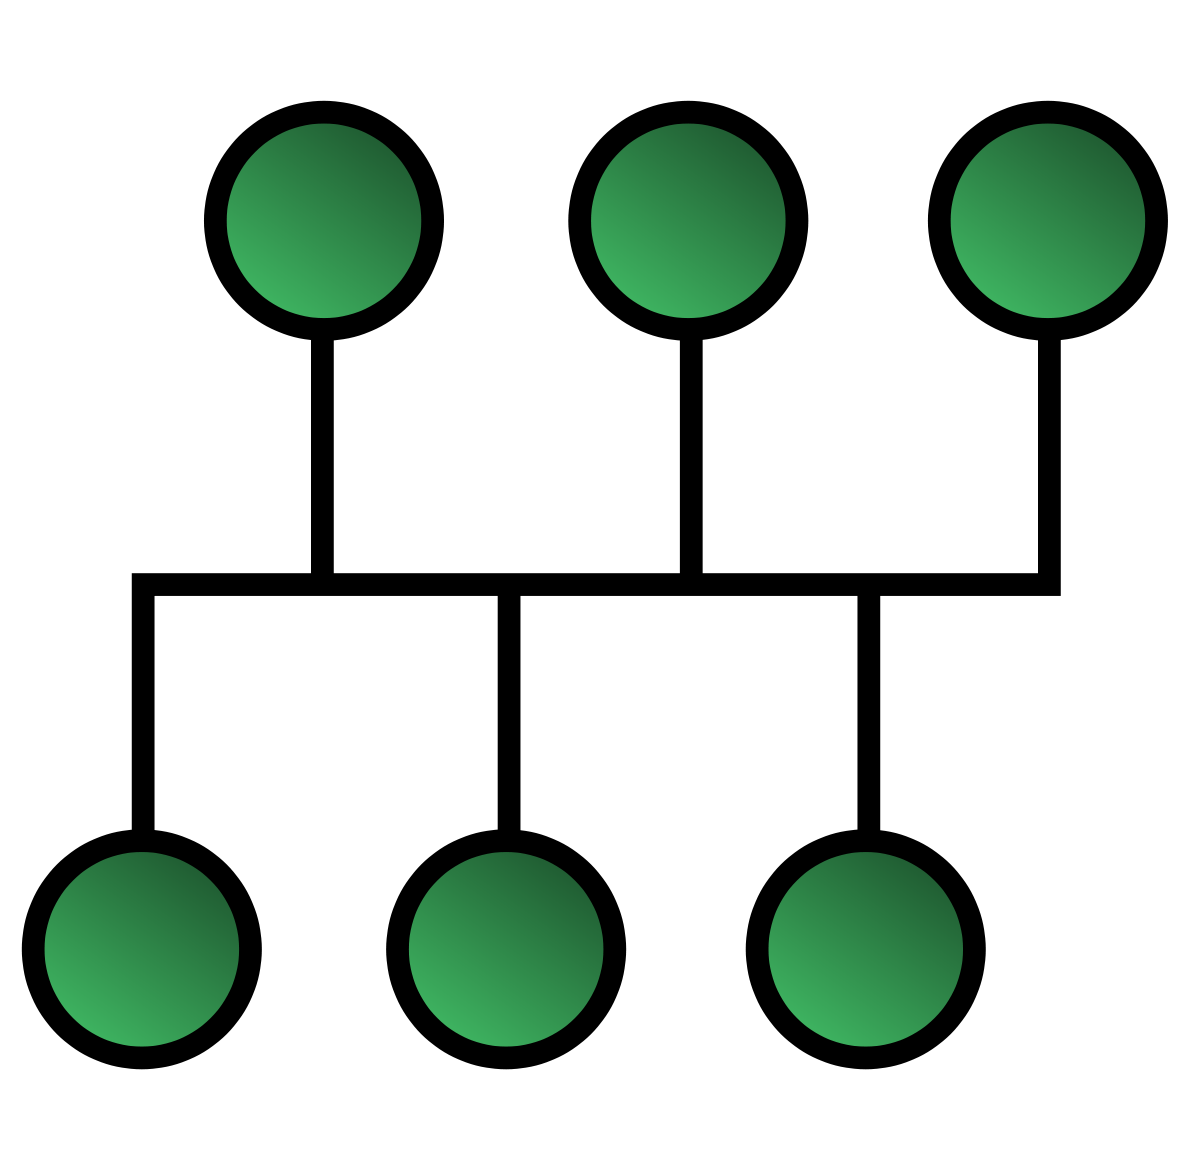
\includegraphics[scale=0.1]{bus}  
		\caption[Topologi \textit{bus}]{Topologi \textit{bus}}
		\label{fig:bus} 
	\end{figure}
	
	\item Topologi \textit{Tree}
	
	Pada topologi \textit{tree}, node-node akan disusun secara hierarki dengan sebuah node yang berada pada level paling atas disebut sebagai \textit{root node}.  \textit{Root node} akan terhubung dengan satu atau lebih node yang levelnya dibawah sehingga \textit{root node} akan bertindak sebagai komunikasi utama (Gambar~\ref{fig:tree}). Penggunaan topologi \textit{tree} lebih mudah untuk melakukan identifikasi dan meminimalisir kesalahan. Kelemahan dari topologi ini adalah topologi ini akan semakin sulit dikonfigurasi seiring jika ukuran \textit{tree} yang sangat besar dan banyaknya \textit{level tree} yang ada.
	
	\begin{figure}[H] 
		\centering  
		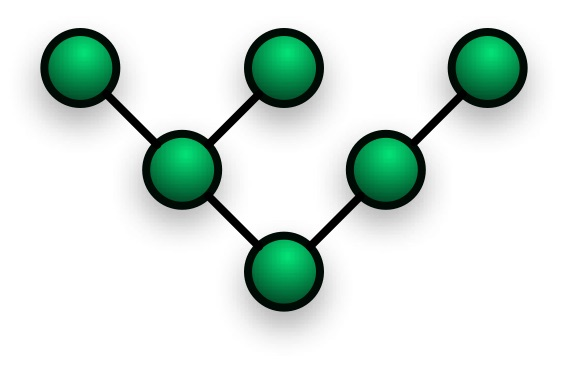
\includegraphics[scale=0.3]{tree}  
		\caption[Topologi \textit{tree}]{Topologi \textit{tree}}
		\label{fig:tree} 
	\end{figure}
	
	\item Topologi \textit{Star}
	
	Topologi \textit{star} memiliki sebuah node yang berada di tengah sebagai \textit{hub} atau \textit{switch} yang biasa disebut \textit{central node} (Gambar~\ref{fig:star}). Setiap node-node akan terhubung dengan \textit{central node} dan melakukan komunikasi ke node lain melalui \textit{central node} ini. \textit{Central node} yang telah mendapatkan pesan dari node pengirim akan meneruskan pesannya ke node tujuan. Apabila \textit{central node} mengalami kerusakan, maka tidak akan terjadinya komunikasi antar node karena segala komunikasi harus dilakukan melalui \textit{central node}.
	
	\begin{figure}[H] 
		\centering  
		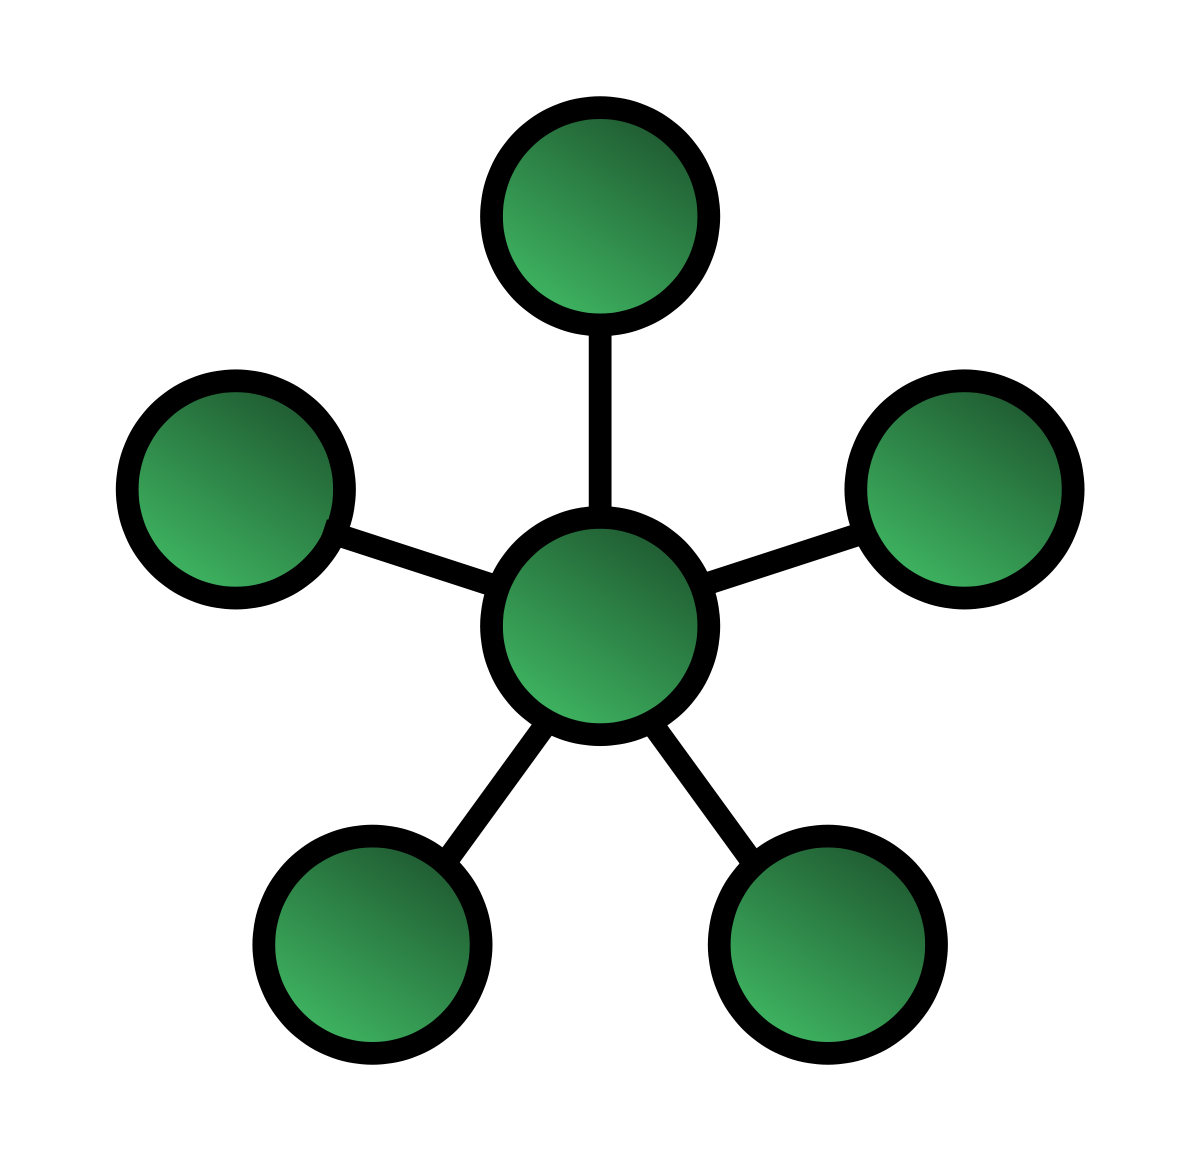
\includegraphics[scale=0.1]{star}  
		\caption[Topologi \textit{star}]{Topologi \textit{star}}
		\label{fig:star} 
	\end{figure}
	
	\item Topologi \textit{ring}
	
	Jaringan topologi \textit{ring} berbentuk rangkaian node yang saling terhubung dengan dua node terdekat lainnya sehingga akan berbentuk seperti lingkaran atau cincin (Gambar~\ref{fig:ring}). Pada topologi \textit{ring}, node akan mengirimkan pesan kemudian akan diteruskan ke node tetangganya sampai menemukan node tujuan yang akan dikirimkan pesan. Kekurangannya adalah salah satu node mati maka komunikasi jaringannya akan mati. Masalah ini dapat diatasi dengan membuat sebuah node tidak hanya dapat melakukan komunikasi satu arah melainkan ke arah sebaliknya.
	
	\begin{figure}[H] 
		\centering  
		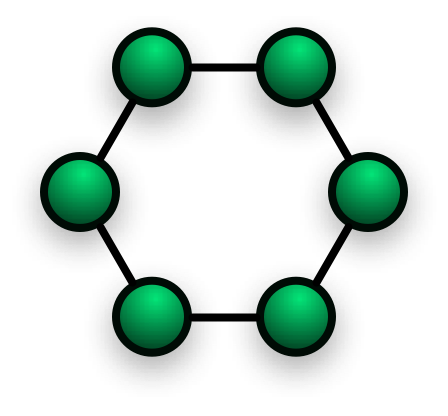
\includegraphics[scale=0.3]{ring}  
		\caption[Topologi \textit{ring}]{Topologi \textit{ring}}
		\label{fig:ring} 
	\end{figure}  
	
	\item Topologi \textit{Mesh}
	
	Topologi mesh dibagi menjadi dua jenis yaitu partially connected mesh dan fully connected mesh. Perbedaannya kedua jenis ini adalah hubungan antar node, pada partially connected mesh, node dapat terhubung dengan satu atau lebih node lainnya (Gambar~\ref{fig:partial}). Sedangkan fully connected mesh, setiap node harus terhubung dengan semua node-node lain yang ada pada sebuah jaringan (Gambar~\ref{fig:full}). 
	
	\begin{figure}[H] 
		\centering  
		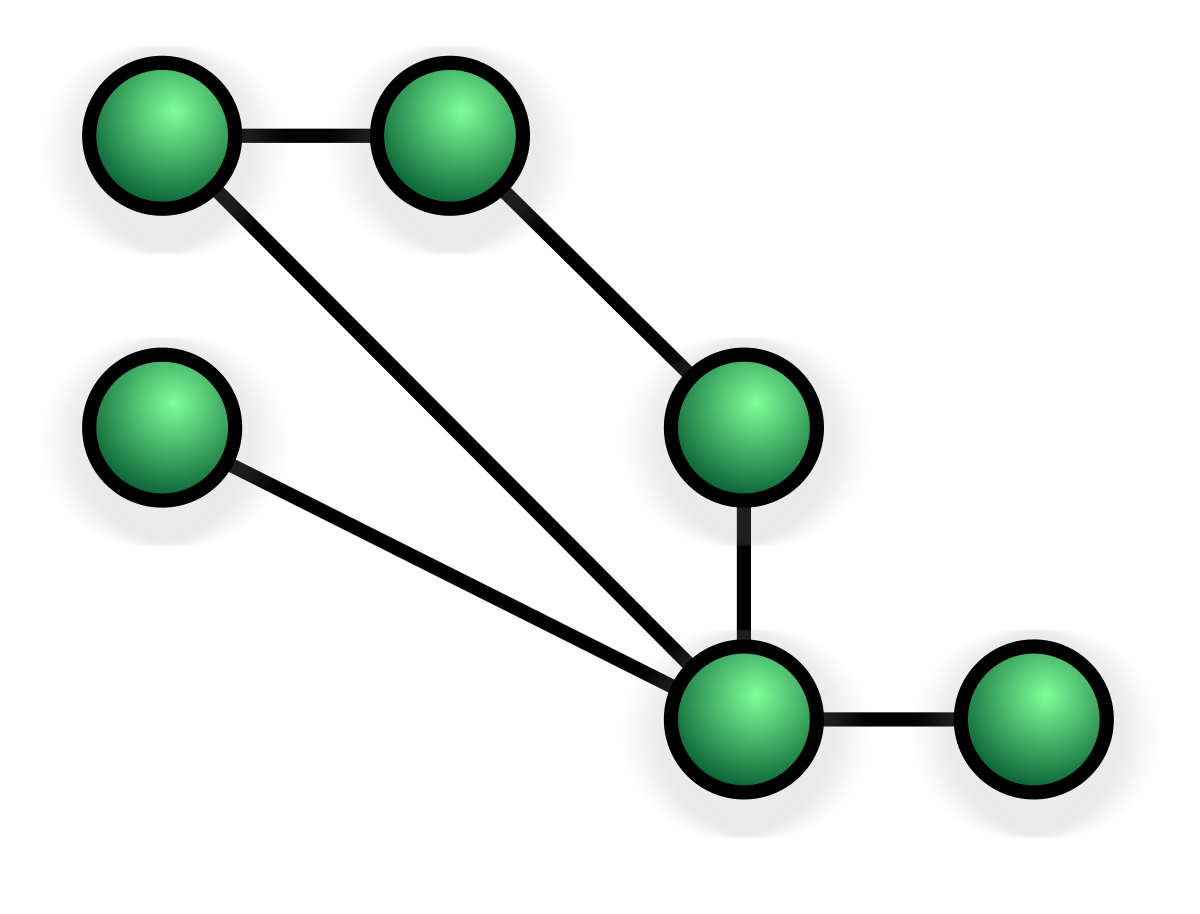
\includegraphics[scale=0.15]{partial}  
		\caption[Topologi \textit{partially connected mesh}]{Topologi \textit{partially connected mesh}}
		\label{fig:partial} 
	\end{figure}  
	
	\begin{figure}[H] 
		\centering  
		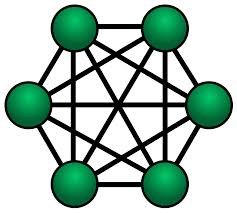
\includegraphics[scale=0.4]{full}  
		\caption[Topologi \textit{fully conneted mesh}]{Topologi \textit{fully conneted mesh}}
		\label{fig:full} 
	\end{figure}  
	
\end{itemize}
	
\subsection{Protokol \textit{Wireless Sensor Network}}
\label{protokol}
\textit{Wireless Sensor Network} memiliki lima layer protokol yaitu \textit{physical layer}, \textit{data link layer}, \textit{network layer}, \textit{transport layer} dan \textit{application layer} (Gambar~\ref{fig:layer}). Selain itu, protokol \textit{Wireless Sensor Network} juga dibagi menjadi 3 grup manajemen yaitu \textit{power management plane}, \textit{connection management plane} dan \textit{task management plane}. \textit{Power management plane} bertanggung jawab untuk mengatur tingkat kekuatan sebuah sensor untuk melakukan \textit{sensing}, memproses data dan melakukan komunikasi. \textit{Connection management plane} bertanggung jawab untuk melakukan konfigurasi terhadap node sensor yang terkait dengan koneksi antar node sensor. \textit{Task management plane} bertanggung jawab untuk pembagian tugas diantara node sensor dalam melakukan \textit{sensing} agar energi yang digunakan efektif dan efisisen.

\begin{figure}[H] 
		\centering  
		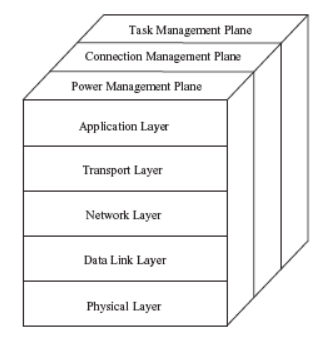
\includegraphics[scale=0.8]{layer}  
		\caption[Layer pada \textit{Wireless Sensor Network}]{Layer pada \textit{Wireless Sensor Network}}
		\label{fig:layer} 
	\end{figure}
	
\begin{itemize}
	\item \textit{Physical layer}
	
	\textit{Physical layer} bertanggung jawab untuk mengubah \textit{bit stream} dari \textit{data link layer} menjadi sinyal agar bisa melakukan transmisi melalui media komunikasi yang tersedia. Pengubahan ini dilakukan agar transmisi dapat dilakukan melalui \textit{transceiver}. Salah satu cara yang bisa digunakan adalah menggunakan \textit{Radio Frequency} (RF). \textit{Radio Frequency} sering dipakai karena biaya yang dikeluarkan murah dan ukuran perangkat yang kecil.	
	
	\item \textit{Data Link layer}
	
	\textit{Data Link layer} bertanggung jawab untuk melakukan \textit{multiplexing} pada aliran data, membentuk \textit{data frame}, mendeteksi \textit{data frame}, \textit{medium access}, and \textit{error control}. Data Link layer juga memiliki proses yang penting yaitu \textit{Medium Access Control} (MAC). Protokol MAC ini bertindak untuk melakukan kontrol terhadap akses media yang dilakukan oleh node sensor dan mencegah terjadinya adanya paket yang bertabrakan.  
	
	\item \textit{Network layer}
	
	\textit{Network layer} bertanggung jawab untuk melakukan \textit{routing} dari node sensor ke \textit{sink node}. Network layer juga merupakan lapisan yang menyediakan jalur komunikasi jaringan sehingga \textit{network layer} bertugas untuk menentukan jenis komunikasi antar node yang digunakan apakah jenis yang digunakan \textit{single hop} atau \textit{multi hop}. 	
	
	\item \textit{Transport layer}
	
	\textit{Transport layer} bertanggung jawab untuk pengiriman data yang \textit{reliable} antar node sensor ke node sensor lainnya atau ke \textit{sink node}. Pengiriman data pada \textit{Wireless Sensor Network} terbagi menjadi dua jenis, yaitu \textit{\textbf{upstream}} dan \textit{\textbf{downstream}}. Kedua jenis ini dibedakan berdasarkan dari asal pengirim dan penerima data. \textbf{Upstream} merupakan node sensor mengirimkan data \textit{sensing} ke \textit{sink node}. Sedangkan \textit{\textbf{downstream}}, \textit{sink node} akan mengirimkan perintah-perintah ataupun \textit{query} ke setiap node sensor yang ada. Setiap jenis pengiriman, kebutuhan \textit{reliability} nya berbeda-beda. Pada \textit{upstream}, \textit{reliable} data dapat ditoleransi karena node sensor mengirimkan data ke sink node secara berulang-ulang sehingga data yang hilang dapat dikoreksi. Pada \textit{downstream}, tidak dapat ditoleransi karena jika data yang dikirimkan tidak \textit{reliable}, maka aplikasi tidak dapat dijalankan.
	
	\item \textit{Application layer}
	
	\textit{Application layer} bertanggung jawab untuk manajemen lalu lintas dan menyediakan antar muka perangkat lunak untuk berbagai aplikasi yang menerjemahkan data dalam bentuk yang dapat dimengerti atau mengirim \textit{query} untuk mendapatkan informasi tertentu.
\end{itemize}

\section{Accelerometer \cite{fft}}
\label{accelerometer}
Salah satu sensor yang terdapat pada node sensor adalah sensor \textit{accelerometer}. \textit{accelerometer} adalah alat yang mengukur \textit{linear acceleration}. Accelerometer memiliki kemampuan untuk mengukur akselerasi, kemiringan, dan getaran statis atau dinamis pada 1 sumbu saja \textit{x/y/z} yang biasa disebut \textit{single axis} atau pada 2 sumbu contohnya \textit{(x,y)} atau \textit{(x,z)} atau \textit{(y,z)} yang biasa disebut dengan \textit{two axis} ataupun 3 sumbu yaitu \textit{(x,y,z)} yang disebut three axis. Sensor \textit{accelerometer} dibagi menjadi 2 jenis yaitu:

\begin{itemize}
	\item \textit{Absolute accelerometer}
	
	\textit{accelerometer} ini terpasang langsung pada objek yang akan diukur.
	
	\item \textit{Relative accelerometer}
	
	\textit{accelerometer} ini mengukur jarak antara objek yang diukur dan titik acuan yang stabil atau bergerak dengan konstan. \textit{accelerometer} ini sering digunakan untuk mengukur getaran dari jarak tertentu.	
\end{itemize}

\section{Fourier Transform}
Fourier Transform adalah sebuah teknik yang digunakan untuk menguraikan sinyal menjadi sinusoids. Sinyal yang diuraikan terdapat sinyal yang bersifat \textit{continous} atau sinyal bersifat discrete, periodic ataupun aperiodic. Sinyal yang bersifat periodic memiliki pola sinyal yang berulang-ulang sedangkan aperiodic memiliki pola yang tidak berulang. Berdasarkan jenis sinyal yang diurai, \textit{Fourier Transform} dibagi menjadi 4 kategori (Gambar~\ref{fig:fourier}).

\begin{figure}[H] 
		\centering  
		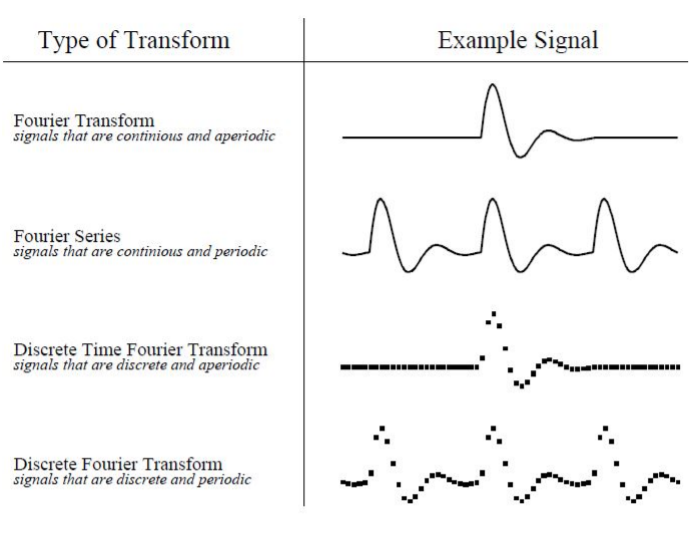
\includegraphics[scale=0.8]{fourier}  
		\caption[Kategori \textit{Fourier Transform} dan contoh bentuk sinyal]{Kategori \textit{Fourier Transform} dan contoh bentuk sinyal}
		\label{fig:fourier} 
\end{figure}

\subsection{Discrete Fourier Transform (DFT)}
\textit{Discrete Fourier Transform} memiliki 2 versi yaitu menggunakan bilangan \textit{real} dan menggunakan bilangan \textit{complex}. \textit{Discrete Fourier Transform} yang menggunakan bilangan complex dapat dikembangkan menjadi \textit{Fast Fourier Transform} \ref{fft} dan akan memiliki persamaan seperti pada persamaan \ref{persamaan1}

\begin{equation}\label{persamaan1}
X(k)=\sum_{n=0}^{N-1} x(n) \times e^{-j\left(\frac{2 \pi}{N}\right) n k}
\end{equation}

Pada persamaan \ref{persamaan1}, variabel N merupakan jumlah sampel, $x(n)$ merupakan input sinyal pada domain waktu, dan X(k) merupakan hasil keluaran sinyal pada domain frekuensi.

\subsection{Fast Fourier Transform (FFT)}\label{fft}
\textit{Fast Fourier Transform} adalah teknik DFT yang lebih efisien. FFT memiliki cara perhitungan DFT yang lebih cepat dan memiliki hasil yang sama dengan hasil DFT. Salah satu contoh dari algoritma FFT adalah \textit{Cooley-Tukey Algorithm}.

\textit{Cooley-Tukey Algorithm} ini terdapat 2 jenis proses yaitu \textit{Decimation in Time} (DIT) dan \textit{Decimation in Frequency} (DIF). Jika masukan dari sinyal pada proses perhitungan adalah domain waktu, maka akan diproses dengan DIT sedangkan jika masukan dari sinyal pada proses perhitungan adalah domain frekuensi, maka akan diproses dengan DIF. DIT akan mengubah sinyal dari domain waktu menjadi domain frekuensi sedangkan DIF akan mengubah sinyal dari domain frekuensi menjadi domain waktu. Setiap masukan dari proses DIT maupun DIF harus diurutkan dalam \textit{bit reverse} agar hasil keluarannya dalam urutan yang tepat. Proses DIT dapat dilihat pada \ref{fig:dit} dan contoh visual dari DIT dengan panjang FFT 8 pada (Gambar \ref{fig:fft}

\begin{figure}[H] 
		\centering  
		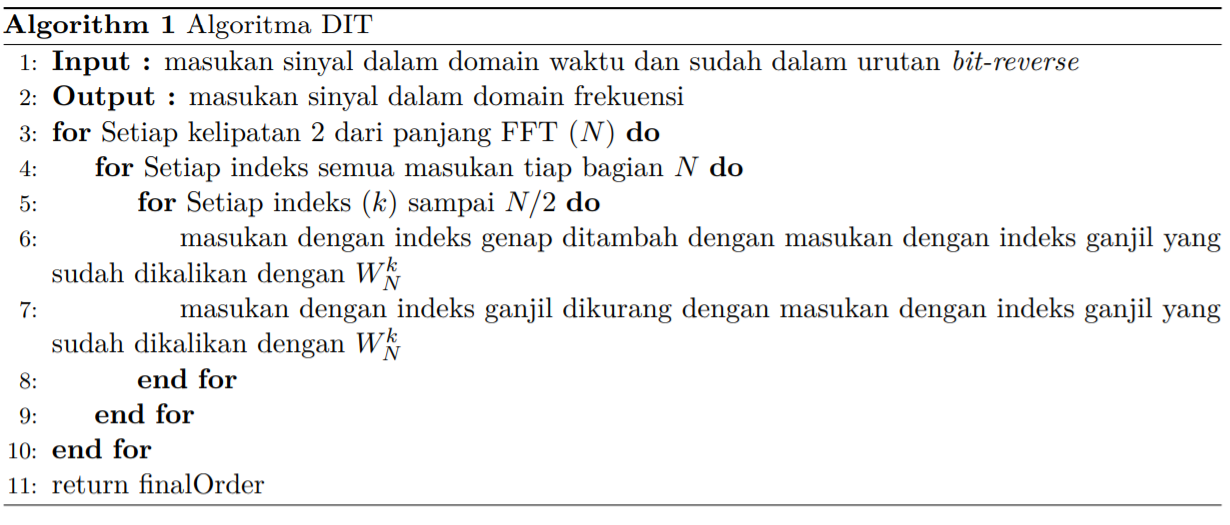
\includegraphics[scale=0.5]{dit}  
		\label{fig:dit} 
\end{figure}

\begin{equation}\label{twiddle}
W_{N}^{k}=e^{-j\left(\frac{2 \pi k}{N}\right)}
\end{equation}

Persamaan \ref{twiddle} disebut juga dengan \textit{twiddle factor}. Nilai k pada persamaan ini adalah indeks bernilai sampai dengan N/2.

\begin{table}[H]
	\centering
	\resizebox{300px}{!}{
    	\begin{tabular}{|c|c|c|c|}
    		\hline 
    		Index & Binary & Bit-reversed Binary & Bit-reversed Index \\ 
    		\hline 
    		0 & 000 & 000 & 0 \\ 
    		\hline
    		1 & 001 & 100 & 4 \\
    		\hline
    		2 & 010 & 010 & 2 \\
    		\hline 
    		3 & 011 & 110 & 6 \\
    		\hline 
    		4 & 100 & 001 & 1 \\
    		\hline 
    		5 & 101 & 101 & 5 \\
    		\hline
    		6 & 110 & 011 & 3 \\
    		\hline 
    		7 & 111 & 111 & 7 \\
    		\hline
    	\end{tabular}
	}
	\caption{Tabel contoh \textit{bit reverse} dari indeks 0 sampai 7}
	\label{contohbit}
\end{table}

\begin{figure}[H] 
		\centering  
		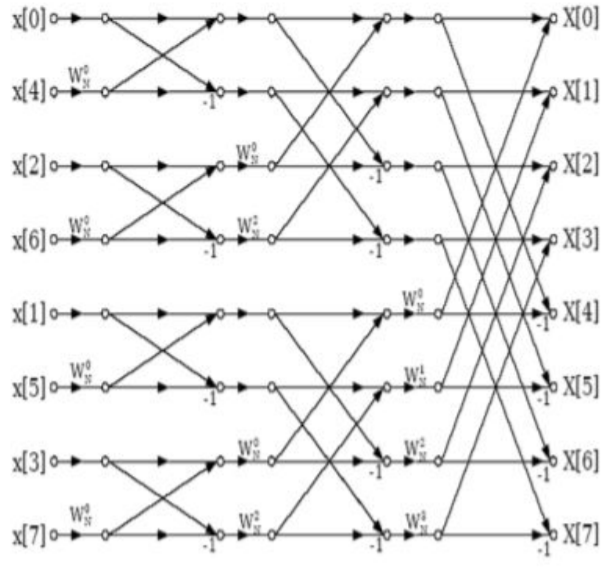
\includegraphics[scale=0.4]{visualDIT}  
		\caption{Contoh visual \textit{Decimation In Time} dengan panjang 8}
		\label{fig:fourier} 
\end{figure}



\section{PreonVM}
\label{preonvm}
PreonVM adalah \textit{virtual machine} (VM) yang berasal dari VIRTENIO untuk digunakan dalam sistem \textit{embedded} dengan sumber daya yang sangat rendah\footnote{https://www.virtenio.com/en/portfolio-items/preonvm/}. \textit{Virtual machine} PreonVM ini sudah sangat optimal dan tidak memerlukan sistem operasi tambahan dan berjalan langsung pada mikrokontroler. Dengan PreonVM, \textit{developer} dapat membuat aplikasi sensor dengan mudah menggunakan bahasa Pemograman Java yang mengumpulkan data-data (hasil \textit{sensing}) dari sensor. API pada PreonVM mendukung antarmuka radio sesuai dengan IEEE 802.15.4.

\subsection{Fitur PreonVM}
Fitur-fitur yang dimiliki oleh PreonVM sebagai berikut:
\begin{itemize}
	\item Aplikasi dibangun dengan Bahasa Pemrograman Java
	\item Mendukung tipe data pada Java seperti \textit{char}, \textit{byte}, \textit{int}, \textit{long}, \textit{float}, atau \textit{double}
	\item Jumlah \textit{thread} yang tidak terbatas
	\item \textit{System properties} untuk konfigurasi aplikasi
	\item \textit{Garbage collection} dengan \textit{memory defragmentation}
	\item \textit{Exception handling} (\textit{try}, \textit{catch}, \textit{Exception}, atau \textit{Runtime Exception})
\end{itemize}

\subsection{Kelebihan PreonVM}
Kelebihan PreonVM adalah PreonVM menggunakan \textit{object-oriented programming} menggunakan bahasa pemrograman Java pada \textit{virtual} \textit{machine} nya untuk \textit{embeed-system}. PreonVM juga dioptimasi agar aplikasi dapat dijalankan 8-bit sampai 32-bit \textit{microcontroller} dengan 8KB RAM dan 128KB Flash minimum. \textit{Virtual Machine} pada PreonVM dapat membuat aplikasi dapat berjalan secara sendiri pada arsitektur yang digunakan. Sehingga aplikasi Java yang dibuat dapat dijalankan pada arsitektur yang berbeda-beda tanpa harus dijalankan (Gambar~\ref{fig:preon}).  

\begin{figure}[H] 
		\centering  
		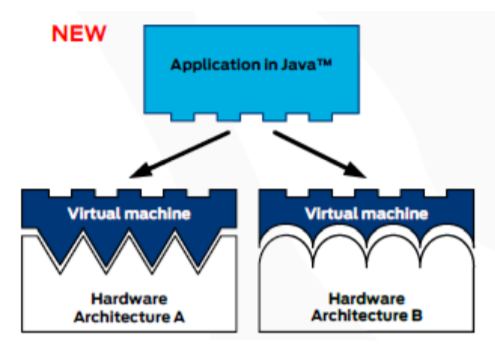
\includegraphics[scale=0.6]{preon}  
		\caption[\textit{Virtual Machine} yang membuat aplikasi dapat dijalankan secara independen]{\textit{Virtual Machine} yang membuat aplikasi dapat dijalankan secara independen}
		\label{fig:preon} 
\end{figure}
	
\subsection{Class Library PreonVM}
PreonVM memiliki 2 \textit{package} yaitu \textit{package} dari Virtenio itu sendiri dan \textit{package} dari Java. \textit{Package} yang disediakan oleh Virtenio dibagi lagi menjadi beberapa bagian diantaranya adalah \textit{Route Packages}, \textit{Radio Packages} dan \textit{Other Virtenio Packages}. Sedangkan \textit{package} yang dari Java terdiri dari \textit{Java Related Packages}. Berikut ada tabel-tabel package yang disediakan:\footnote{https://virtenio/com/assets/vm/javadoc/overview-summary.html}

\begin{table}[H]
	\centering
	\caption{Tabel Route Packages}
	\resizebox{\textwidth}{!}{
		\begin{tabular}{|l|l|}
			\hline 
			Package & Deskripsi \\ 
			\hline 
			com.virtenio.route.aodv & Paket yang berisi kelas terkait AODV (Ad Hoc On Demand Vector) Routing  \\ 
			\hline 
		\end{tabular}
	}
\end{table}

\begin{table}[H]
	\centering
	\caption{Tabel Radio Packages}
	\resizebox{\textwidth}{!}{
		\begin{tabular}{|l|l|}
			\hline 
			Package & Deskripsi \\ 
			\hline 
			com.virtenio.radio & Paket yang berisi kelas terkait radio \\ 
			\hline 
			\texttt{ESRTcom.virtenio.radio.ieee\_802\_15\_4} & Paket yang berisi kelas terkait IEEE 802.15.4 \\ 
			\hline 
		\end{tabular}
	}
\end{table}

\begin{table}[H]
	\centering
	\caption{Tabel Other Virtenio Packages}
	\resizebox{\textwidth}{!}{
		\begin{tabular}{|l|l|}
		\hline
		Package & Deskripsi \\
		\hline
		com.virtenio.crypt & Paket yang berisi untuk enkripsi dan dekripsi \\
		\hline 
		com.virtenio.driver & Paket yang berisi drivers untuk berbagai perangkat \\ 
		\hline 
		com.virtenio.driver.adc & Paket yang berisi kelas ADC \textit{driver} \\ 
		\hline 
		com.virtenio.driver.atmodem & Paket yang berisi kelas ATModem \textit{driver} \\ 
		\hline 
		com.virtenio.driver.button & Paket yang berisi kelas \textit{button} \textit{driver} \\ 
		\hline 
		com.virtenio.driver.can & Paket yang berisi kelas CAN \textit{driver} \\ 
		\hline 
		com.virtenio.driver.cpu & Paket yang berisi kelas CPU \textit{driver} \\ 
		\hline 
		com.virtenio.driver.device & Paket yang berisi kelas \textit{device driver} \\ 
		\hline 
		com.virtenio.driver.device.at86rf212 & Paket yang berisi \textit{driver} untuk perangkat AT86RF212 \\ 
		\hline 
		com.virtenio.driver.device.at86rf231 & Paket yang berisi \textit{driver} untuk perangkat AT86RF231 \\ 
		\hline 
		com.virtenio.driver.flash & Paket yang berisi kelas \textit{Flash driver} \\ 
		\hline 
		com.virtenio.driver.gpio & Paket yang berisi kelas GPIO \textit{device driver} \\ 
		\hline 
		com.virtenio.driver.i2c & Paket yang berisi kelas I2C \textit{device driver} \\ 
		\hline 
		com.virtenio.driver.irq & Paket yang berisi kelas IRQ \textit{device driver} \\ 
		\hline 
		com.virtenio.driver.led & Paket yang berisi kelas LED \textit{device driver }\\ 
		\hline 
		com.virtenio.driver.lin & Paket yang berisi kelas LIN \textit{device driver} \\ 
		\hline 
		com.virtenio.driver.onewire & Paket yang berisi kelas OneWire \textit{device driver} \\ 
		\hline 
		com.virtenio.driver.pwm & Paket yang berisi kelas PWM (\textit{pulse-width modulation}) \textit{device driver} \\ 
		\hline 
		com.virtenio.driver.ram & Paket yang berisi kelas FRAM \textit{device driver} \\ 
		\hline 
		com.virtenio.driver.rtc & Paket yang berisi kelas untuk pengaturan jam secara \textit{real-time}, dan \textit{real-counter device driver} \\ 
		\hline 
		com.virtenio.driver.spi & Paket yang berisi kelas SPI (\textit{Serial Peripheral Interface}) \textit{device driver} \\ 
		\hline 
		com.virtenio.driver.sw & Paket yang berisi kelas \textit{switch device driver} \\ 
		\hline 
		com.virtenio.driver.timer & Paket yang berisi kelas \textit{hardware timer device driver} \\ 
		\hline 
		com.virtenio.driver.usart & Paket yang berisi kelas USART \textit{device driver} \\ 
		\hline 
		com.virtenio.driver.watchdog & Paket yang berisi WatchDog \textit{device driver} \\ 
		\hline 
		com.virtenio.io & Paket Virtenio VM yang berisi IO \\ 
		\hline 
		com.virtenio.lib & Paket Virtenio VM yang berisi pengaturan classlib \\ 
		\hline 
		com.virtenio.misc & Paket tambahan Virtenio VM \\ 
		\hline 
		com.virtenio.net &  \\ 
		\hline 
		com.virtenio.vm & \\ 
		\hline 
		com.virtenio.vm.event & Sistem event pada Virtenio VM untuk menangani \textit{event} \textit{asynchronous} dan \textit{synchronous} \\ 
		\hline 
		\end{tabular} 
	}
\end{table}

\begin{table}[H]
	\centering
	\caption{Tabel Java Related Pakcages}
		\begin{tabular}{|l|l|}
			\hline 
			Package & Deskripsi \\ 
			\hline 
			java.io & Paket Java IO \\ 
			\hline 
			java.lang & Paket Java lang \\ 
			\hline
			java.lang.annotation & Paket \textit{Annotation} pada Java \\
			\hline
			java.lang.ref & \\
			\hline
			java.nio & \\
			\hline
			java.nio.channels & \\
			\hline 
			java.text & Paket Java Text \\
			\hline
			java.util & Paket Java \textit{Utility} yang berisi \textit{collection} \\
			\hline
			java.util.regex & Paket Java \textit{Regular Expression} \\
			\hline
		\end{tabular}
\end{table}

\subsection{Preon32}
\label{preon32}
Preon32 merupakan salah satu sensor node buatan VIRTENIO. Preon32 menggunakan PreonVM digunakan sebagai operating software untuk sensor node ini.  Pada umumnya, Preon32 memiliki 5 jenis sensor pada sebuah board. Sensor yang ada antara lain adalah sensor suhu (\textit{temperature sensor}), sensor cahaya (\textit{light intensity sensor}), sensor tekanan udara (\textit{air pressure sensor}), sensor getaran (\textit{acceleration sensor}) dan sensor kelembaban udara (\textit{relative humidity sensor}). Preon32 juga terdapat versi tambahannya dilengkapi dengan sensor untuk mendeteksi \textit{gyroscope} dan medan magnet (Gambar~\ref{fig:preon32}).

\begin{figure}[H] 
		\centering  
		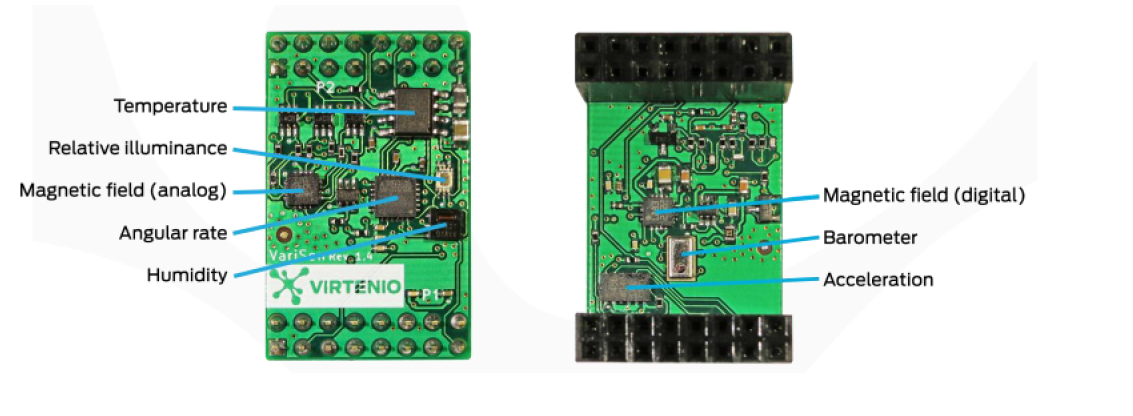
\includegraphics[scale=0.6]{preon32}  
		\caption[Preon32 Board]{Preon32 Board}
		\label{fig:preon32} 
\end{figure}

\subsection{Spesifikasi Sensor-Sensor Preon32}
Berikut spesifikasi sensor-sensor yang terdapat di Preon32:
\begin{itemize}
	\item Sensor suhu (\textit{temperature} sensor)
	\begin{itemize}
		\item Manufacture : Analog Devices
		\item Model : ADT7410
		\item Interface : digital, I2C
		\item Resolution : 16-Bit
		\item Range : -40$^{\circ}$C sampai +105$^{\circ}$C
		\item Accuracy : $\pm$0.5$^{\circ}$C
	\end{itemize}
\end{itemize}

\begin{itemize}
	\item Sensor cahaya (\textit{light intensity} sensor)
	\begin{itemize}
		\item Manufacture : Rohm
		\item Model : BH1715FVC
		\item Interface : digital, I2C
		\item Resolution : 16-Bit
		\item Range : 1 lx to 65355 lx
	\end{itemize}
\end{itemize}

\begin{itemize}
	\item Sensor tekanan udara (\textit{air pressure} sensor)
	\begin{itemize}
		\item Manufacture : Freescale
		\item Model : MPL115A2
		\item Interface : digital, I2C
		\item Resolution : 0,15 kPa
		\item Range : 50 kPa sampai 115 kPa
		\item Accuracy : $\pm$1.0 kPa
	\end{itemize}
\end{itemize}

\begin{itemize}
	\item Sensor getaran (\textit{acceleration} sensor)
	\begin{itemize}
		\item Manufacture : Analog Devices
		\item Model : ADXL345
		\item Interface : digital, SPI
		\item Resolution : 13 Bit per axis
		\item Range : $\pm$16 g, 3 axis
		\item Accuracy : 3,9 mg/LSB
	\end{itemize}
\end{itemize}

\begin{itemize}
	\item Sensor kelembaban udara (\textit{relative humidity} sensor)
	\begin{itemize}
		\item Manufacture : Sensirion
		\item Model : SHT21
		\item Interface : digital, I2C
		\item Resolution : 12-Bit
		\item Range : 0 $\%$RH sampai 100 $\%$RH
		\item Accuracy : $\pm$2,0 $\%$RH (typ.)
	\end{itemize}
\end{itemize}